\hypertarget{ux5173ux95edux65f6ux957f}{%
\subsubsection{关闭时长}\label{ux5173ux95edux65f6ux957f}}

问题:创建和关闭操作(如议题、更改请求或需要支持的问题单)之间需要多少时间?

\hypertarget{ux63cfux8ff0}{%
\paragraph{描述}\label{ux63cfux8ff0}}

关闭时长是指从创建到关闭操作(如议题、更改请求或需要支持的问题单)的总时长。
操作需要具有打开和关闭的状态,比如代码审查进程、问答论坛、问题跟踪系统中经常出现的情况。

相关指标:\href{https://chaoss.community/metric-issue-resolution-duration/}{问题解决时长}

\hypertarget{ux76eeux6807}{%
\paragraph{目标}\label{ux76eeux6807}}

\begin{enumerate}
\def\labelenumi{\arabic{enumi}.}
\tightlist
\item
  确定社区的响应程度,帮助增加包容性,吸引新贡献者并保留现有贡献者。
\item
  找出导致快速或缓慢关闭的操作特征(如寻找最佳实践、改进领域、评估效率)。
\item
  识别对不同社区成员及时响应的偏差。
\item
  检测社区活动的变化(例如,显示潜在的维护者倦怠、贡献多元化的减少)
\item
  了解关闭议题或更改请求的时间与合并成功或失败的关系
\end{enumerate}

\hypertarget{ux5b9eux73b0}{%
\paragraph{实现}\label{ux5b9eux73b0}}

\hypertarget{ux7b5bux9009ux6761ux4ef6}{%
\subparagraph{筛选条件}\label{ux7b5bux9009ux6761ux4ef6}}

\begin{itemize}
\tightlist
\item
  操作的创建者(例如,新贡献者相对于维护者)
\item
  最初关闭,最后关闭
\item
  标签(例如错误与新功能)
\item
  更改请求合并状态(例如,合并时间或没有合并的关闭时间)
\end{itemize}

\hypertarget{ux53efux89c6ux5316ux6548ux679c}{%
\subparagraph{可视化效果}\label{ux53efux89c6ux5316ux6548ux679c}}

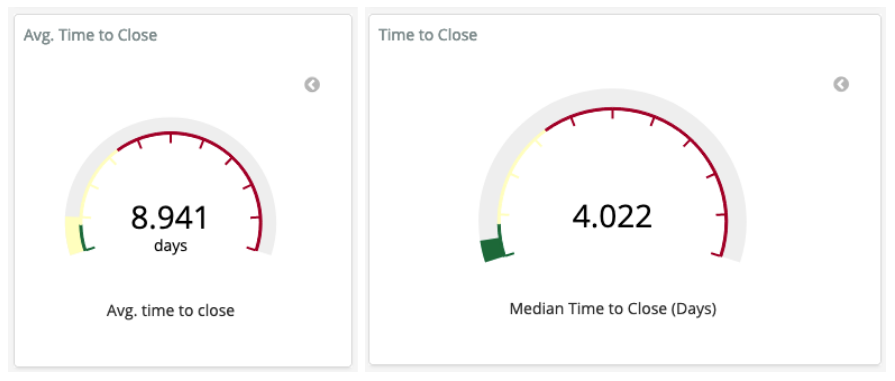
\includegraphics{images/time-to-close_1.png}

\hypertarget{ux63d0ux4f9bux6307ux6807ux7684ux5de5ux5177}{%
\subparagraph{提供指标的工具}\label{ux63d0ux4f9bux6307ux6807ux7684ux5de5ux5177}}

Augur 实现:

\begin{itemize}
\tightlist
\item
  \href{http://augur.osshealth.io/api_docs/\#api-Evolution-Closed_Issue_Resolution_Duration(Repo)}{问题解决时长}
\item
  \href{http://augur.osshealth.io/api_docs/\#api-Evolution-issue-duration-repo}{问题持续时间}
\item
  \href{http://augur.osshealth.io/api_docs/\#api-Evolution-Issue_Response_Time(Repo)}{问题响应时间}
\end{itemize}

GrimoireLab 实现:

\begin{itemize}
\tightlist
\item
  \href{https://chaoss.github.io/grimoirelab-sigils/panels/github-pullrequests-efficiency/}{拉取请求效率}
\item
  \href{https://chaoss.github.io/grimoirelab-sigils/panels/github-issues-efficiency/}{问题效率}
\item
  \href{https://chaoss.github.io/grimoirelab-sigils/panels/efficiency-timing-overview/}{Efficiency:TimingOverview}
\end{itemize}

\hypertarget{ux6570ux636eux6536ux96c6ux7b56ux7565}{%
\subparagraph{数据收集策略}\label{ux6570ux636eux6536ux96c6ux7b56ux7565}}

关闭时长指标可根据项目活动和目标的具体情况而定。
例如,错误报告的关闭时长可能提供与新功能请求的关闭时长不同的信息。
数据收集策略应针对不同的项目目标。 可能影响这些进程的其他变量是:

\begin{itemize}
\tightlist
\item
  问题跟踪系统:如错误报告、蓝图 (OpenStack 专有命名)、用户故事(user
  story)、功能请求、epic等可能会影响事件关闭时长的议题类型。
  优先级或严重性等其他变量可能有助于推进这一事件的关闭速度。
\item
  变更请求流程:这取决于变更请求的平台架构,如 Gerrit、GitHub
  或邮件列表(如 Linux 内核中),并可能根据进程的复杂程度而有所不同。
  例如,新人和经验丰富的高级开发者将以不同的方式开展进程,所需时间或多或少。
\item
  问答论坛:这取决于回答的质量和提问者的意见。
  有效答案会被标记,提问者成功找到自己问题的正确答案后,进程随即关闭。
\end{itemize}

\hypertarget{ux53c2ux8003ux8d44ux6599}{%
\paragraph{参考资料}\label{ux53c2ux8003ux8d44ux6599}}

\begin{itemize}
\tightlist
\item
  ``Practice P.12: Respond to all submissions'',出自``Appendix to:
  Managing Episodic Volunteers in Free/Libre/Open Source Software
  Communities'',Ann Barcomb、Klaas-Jan Stol、Brian Fitzgerald 和 Dirk
  Riehle:\href{https://opus4.kobv.de/opus4-fau/frontdoor/index/index/docId/13519}{https://opus4.kobv.de/opus4-fau/frontdoor/index/index/docId/13519}
\end{itemize}
